\newpage
\section{Критерии вполне ограниченности}
\begin{definition}
	Пространство 
	$$
	c = \{x \in \N \rr \R \mid \exists \lim\limits_{n \rr \infty} = x(\infty) \in \R\}
	$$
	Норма в данном пространстве 
	$$
	\|x\|_\infty = \sup\limits_{n \in \N} |x(n)|
	$$
\end{definition}
\begin{theorem}
	Подмножество $S \subset c$ вполне ограниченно тогда и только тогда когда
	\begin{enumerate}
		\item $S$ --- ограниченно в $c$, то есть $\exists R > 0  \ \forall x \in S \Rightarrow \|x\|_\infty \leq R$
		\item $\forall \eps > 0 \ \exists N \in \N \ \forall x \in S \ \forall n \geq N \Rightarrow |x(n) - x(\infty)| < \eps$
	\end{enumerate}
\end{theorem}
\begin{proof}
	Пусть $S \subset c$ является вполне ограниченным, тогда $S$ --- ограниченно (это верно в любом метрическом пространстве). Теперь покажем второе свойство. По определению $\forall \eps > 0$ существует конечная $\eps$-сеть: 
	$$
	x_1, \dots x_M \in S: S \subset \bigcup_{m=1}^M B_\eps(x_m)
	$$
	Для каждого элемента сети имеем: $\exists x_m(\infty) = \lim\limits_{n \rr \infty} x_m(n) \in \R$, значит
	$$
	\forall m \in \overline{1, M} \ \exists N_m(\eps): \ \forall n \geq N_m |x_m(n) - x_m(\infty)| < \eps
	$$
	Тогда рассмотрим $N = \max\{ n_m \mid m \in \overbrace{1,M}\}$, тогда 
	$$
	\forall x \in S \exists m \in \overbrace{1, M} : x \in B_\eps(x_m) \Rightarrow  \forall n \in \N: \ |x(n) - x_m(n)| \leq \|x_m - x\| < \eps
	$$
	Тогда пользуясь неравенством треугольника получим:
	$$
	\forall x \in S \forall n \geq N: \ |x(n) - x(\infty)| \geq |x(n) - x_m(n)| + |x_m(\infty) - x(\infty)| + |x_m(n) - x(\infty)| \leq 3\eps 
	$$
	Таким образом в необходимую сторону доказано. Докажем достаточность, пусть:
	\begin{enumerate}
		\item $S$ --- ограниченно в $c$, то есть $\exists R > 0  \ \forall x \in S \Rightarrow \|x\|_\infty \leq R$
		\item $\forall \eps > 0 \ \exists N \in \N \ \forall x \in S \ \forall n \geq N \Rightarrow |x(n) - x(\infty)| < \eps$
	\end{enumerate}
	Возьмем $N(\eps)$ из второго условия. определим \glqqконечномерный обрубок\grqq множества $S$:
	$$
	S_\eps = \{(x(1), \dots, x(N(\eps)))^\perp \in \R^{N(\eps)} \mid x \in S\}
	$$
	Так как множество $S$ ограниченно $S_\eps$ содержится $N(\eps)$-мерном параллелепипеде 
	$$
	S_\eps \subset P_R = \{(z(1), \dots, z(N(\eps)))^\perp  \in \R^{N(\eps)}\mid \forall n \in \overline{1, N} \ |z(n)| \leq R \}
	$$
	Тогда разрежем данный параллелепипед на маленькие кубики c длинной стороны не больше $\eps$: 
	\begin{center}
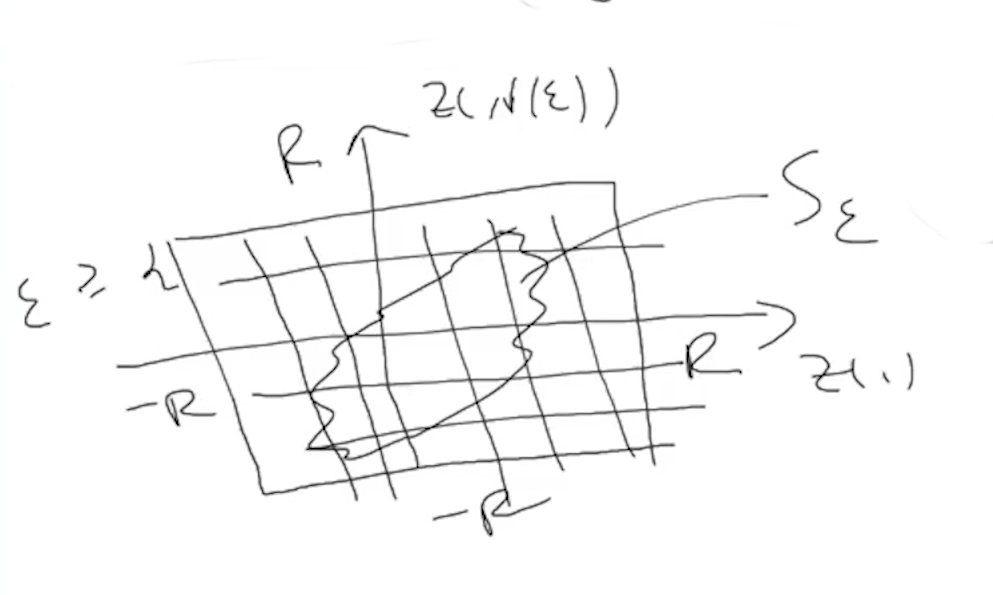
\includegraphics[scale=0.4]{pic/2022-01-22_16-29}
	\end{center}
	
	Определим множество кубиков, пересекающихся с множеством $S_\eps$:
	$$
	G = \{ \square : \square \cap S_\eps \neq \varnothing\}
	$$
	Тогда 
	$$
	\forall \square \in G : \exists x_\square \in S: (x_\square(1), \dots x_\square(N(\eps)))^\perp \in \square \cap S_\eps 
	$$
	Таким образом $C_\eps = \{x_\square \mid \square \in G \}$ --- это конечное подмножество $S$ (будущая сеть). Внутри конечномерного параллелепипеда мы воспользуемся ограниченностью, а оставшиеся координаты оценим с помощью второго условия. Приступим: 
	$$
	\forall x \in S \Rightarrow (x(1), \dots, x(N(\eps)))^\perp \in S_\eps \subset P_R \Rightarrow \exists \square \ni (x(1), \dots, x(N(\eps)))^\perp \in S_\eps
	$$
	Значит $\square \in G$, тогда для этого кубика есть уже заготовленная точка $x_\square$ из конечного множества, тогда так как ребро каждого кубика не больше $\eps$ получаем:
	$$
	\forall n \in \overline{1, N(\eps)}: \ |x(n) - x_\square(n)| \leq \eps 
	$$
	В силу второго условия:
	$$
	\forall n \geq N(\eps): \ |x(n) - x(\infty)| \leq \eps, \ |x_\square(n) - x_\square(\infty)| \leq \eps
	$$
	То есть координаты после $N(\eps)$ далеко не разбегаются:
	$$
	|x(n) - x(N(\eps))| \leq |x(n) - x(\infty)| + |x(N(\eps)) - x(\infty)| \leq 2\eps
	$$
	Аналогично для $x_\square$: $|x_\square(n) - x_\square(N(\eps)))| < \eps$, таким образом получаем:
	$$
	\forall n > N(\eps): \ |x(n)-x_\square(n)| \leq |x(n) - x(N(\eps))| + |x(N(\eps)) - x_\square(N(\eps))| + |x_\square(N(\eps) - x_\square(n))| \leq 2\eps + \eps + 2\eps = 5\eps
	$$
	Таким образом мы оценили хвост и общая оценка:
	$$\|x- x_\square\|_\infty \leq |x(n) - x_\square| \leq 5\eps$$
	Таким образом $C_\eps$ --- конечная $5\eps$-сеть. Значит $S$ --- вполне ограничено.
\end{proof}
\begin{definition}
	Пространство $C(K)$ --- множество непрерывных на компакте $K$ функций $f : K \rr \R$ по умолчанию имеет норму:
	$$
	\|f\|_c  = \sup\limits_{x \in K} |f(x)| = \max\limits_{x \in K}|f(x)|
	$$
\end{definition}
\begin{theorem}[Арцела-Асколе]\label{th:arzela}
	Пусть $(K, \rho)$ --- компактное метрическое пространство. Тогда $S \subset C(K)$ --- вполне ограниченно тогда и только тогда когда
	\begin{enumerate}
		\item $S$ --- ограниченно в $C(K)$, то есть $\exists R > 0 \forall f \in S \Rightarrow \|f\|_c \leq R$
		\item $S$ --- равностепенно непрерывно: 
		$$
		\forall \eps > 0 \exists \delta = \delta(\eps): \forall f \in S, \ \forall x, y \in K : \rho(x,y) \leq \delta \Rightarrow |f(x) - f(y)| \leq \eps 
		$$
	\end{enumerate}
\end{theorem}
\begin{proof}
	Необходимость. $S$ --- вполне ограниченно $\Rightarrow$ $S$ --- ограниченно. Так же имеем конечную $\eps$-сеть:
	$$
	\forall \eps > 0 \exists f_1, \dots, f_M \in S: \ S \subset \bigcup_{m = 1}^M B_\eps(f_m)
	$$
	Тогда по теореме кантора для каждого шара:
	$$
	\forall m \in \overline{1, M} \ \exists \delta_m(\eps) > 0 : \ \forall x,y \in K \ \rho(x,y) \leq \delta_m \Rightarrow |f_m(x) - f_m(y)| \leq \eps 
	$$
	Тогда положив $\delta = \min\limits_{m \in \overline{1, M}} \delta_m$ получим, что $\delta$ зависит только от $\eps$ и 
	$$
	\forall m \in \overline{1, M}, \ \forall x,y \in K:  \rho(x,y) < \delta \Rightarrow |f_m(x) - f_m(y)| \leq \eps 
	$$
	Тогда, пользуясь неравенством треугольника, получаем:
	$$
	\begin{gathered}
	\forall f \in S: \exists m \in \overline{1, M}: f \in B_\eps(f_m) \Rightarrow \forall x,y \in K, \ \rho(x,y) < \delta: \\ \ |f(x) - f(y)| \leq |f(x) - f_m(x)| + |f_m(x) - f_m(y)| + |f_m(y) - f(y)| \leq \eps + \eps + \eps = 3\eps
	\end{gathered}
	$$
	Таким образом необходимость доказана. Докажем необходимость. Пусть выполнено:
	\begin{enumerate}
		\item $S$ --- ограниченно в $C(K)$, то есть $\exists R > 0 \forall f \in S \Rightarrow \|f\|_c \leq R$
		\item $S$ --- равностепенно непрерывно: 
		$$
		\forall \eps > 0 \exists \delta = \delta(\eps): \forall f \in S, \ \forall x, y \in K : \rho(x,y) \leq \delta \Rightarrow |f(x) - f(y)| \leq \eps 
		$$
	\end{enumerate}
	По аналогии с предыдущей теоремой для числа $\delta(\eps)$ в компактом метрическом пространстве $(K, \rho)$ мы имеем конечную $\delta(\eps)$-сеть:
	$$
	x_1, \dots, x_M \in K: K = \bigcup_{m=1}^M B_\delta(\eps)^K(x_m) 
	$$
	Тогда построим:
	$$
	S_\eps = \{(f(x_1), \dots f(x_M))^\perp \in \R^M \mid f \in S\}
	$$
	Тогда в силу ограниченности $S$:
	$$
	S_\eps \subset P_R = \{(z_1, \dots, z_M) \in R^M \mid \forall n \in \overline{1, M}: |z(n)| \leq R \}
	$$
	\newpage
	Повторяя предыдущее доказательство режем данный кубик на кубики со стороной не больше $\eps$
	\begin{figure}[h!]
		\centering
		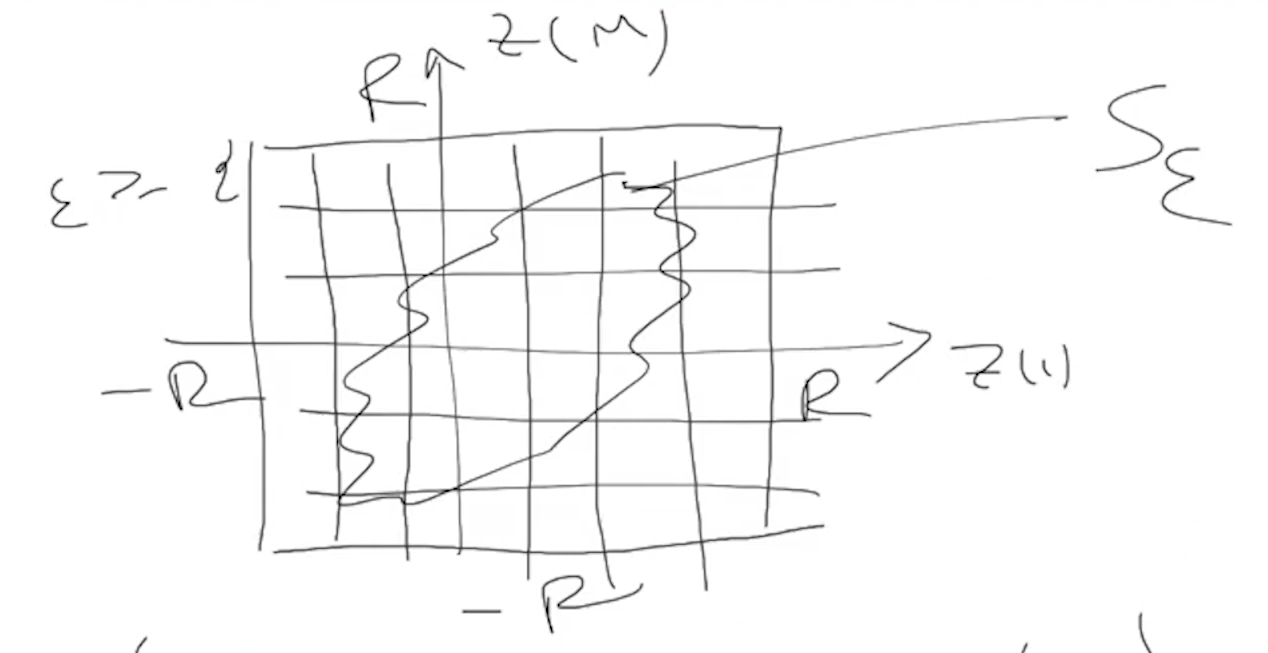
\includegraphics[width=0.7\linewidth]{pic/screenshot001}
		\caption{}
		\label{fig:screenshot001}
	\end{figure}
Рассмотрим: $G = \{\square : \square \cap S_\eps \neq \varnothing \}$ этих кубиков конечное число, тогда рассматриваем соответствующие $C_\eps = \{f_\square \in S \mid \square \in G\}$ --- тоже конечно. Тогда
$$
\forall f \in S: (f(x_1), \dots, f(x_M))^\perp \in S_\eps \subset P_R \Rightarrow \exists f_\square: \forall m \in \overline{1, M}: |f(x_m) - f_\square(x_m)| \leq \eps
$$
Тогда 
$$\forall x \in K 	\ \exists m \in \overline{1, M}: \ x \in B_{\delta(\eps)}^K(x_m)$$
То есть $\rho(x,x_m) \leq \delta(\eps)$ и тогда
$$
|f(x) - f_\square(x)| \leq |f(x) - f(x_m)| + |f(x_m) - f_\square(x_m)| + |f_\square(x_m) = f_\square(x)| \leq 3\eps \Rightarrow \|f - f_\square\|_c \leq 3\eps
$$
Таким образом $S$ --- вполне ограниченно. 
\end{proof}